\documentclass[11pt,a4paper,twocolumn]{article}
\usepackage[margin=0.7in, columnsep=0.25in]{geometry}
\usepackage{setspace}
\usepackage{graphicx}
\usepackage{amsmath, amssymb}
\usepackage{booktabs}
\usepackage{longtable}
\usepackage{caption}
\usepackage{float}
\usepackage{hyperref}
\usepackage{enumitem}
\usepackage{xcolor}
\usepackage{tabularx}
\usepackage{natbib}
\usepackage{tikz}
\usepackage{multirow}
\usepackage{listings}
\usepackage{adjustbox}
\usepackage{algorithm}
\usepackage{algorithmic}
\usepackage{stfloats}
\usetikzlibrary{shapes.geometric, arrows, positioning, fit, calc, backgrounds}

\lstset{
  basicstyle=\ttfamily\small,
  frame=single,
  breaklines=true,
  backgroundcolor=\color{gray!10},
}

% Custom colors
\definecolor{darkblue}{RGB}{0,51,102}
\definecolor{codegreen}{RGB}{0,128,0}

\hypersetup{
    colorlinks=true,
    linkcolor=darkblue,
    citecolor=darkblue,
    urlcolor=darkblue,
}

% IEEE-style section numbering: I, II, III / A, B, C / 1, 2, 3
\renewcommand{\thesection}{\Roman{section}}
\renewcommand{\thesubsection}{\Alph{subsection}}
\renewcommand{\thesubsubsection}{\arabic{subsubsection}}

% IEEE-style section title formatting
\makeatletter
\renewcommand{\section}{\@startsection{section}{1}{\z@}%
  {-3ex \@plus -1ex \@minus -.2ex}%
  {2.0ex \@plus.2ex}%
  {\normalfont\large\bfseries\centering\MakeUppercase}}
\renewcommand{\subsection}{\@startsection{subsection}{2}{\z@}%
  {-2.75ex\@plus -1ex \@minus -.2ex}%
  {1.00ex \@plus .2ex}%
  {\normalfont\normalsize\bfseries\itshape}}
\renewcommand{\subsubsection}{\@startsection{subsubsection}{3}{\z@}%
  {-2.75ex\@plus -1ex \@minus -.2ex}%
  {1.ex \@plus .2ex}%
  {\normalfont\normalsize\itshape}}
\makeatother

\begin{document}

\twocolumn[{%
\begin{center}

{\fontsize{22}{26}\selectfont\textbf{Intelligent Drone Navigation and Fleet Optimization for Last-Mile Delivery in Regulated Indian Airspace}\par}

\vspace{0.6cm}

{\normalsize
Dr. Vipul Kumar Mishra*, Aditya Acharya*, Harphool Singh*, Pradeep Kumar*, Vishvendra*
\par}

\vspace{0.15cm}

{\small
*Department of Artificial Intelligence and Data Science \\
Gati Shakti Vishwavidyalaya, Vadodara, India -- 390004
\par}

\vspace{0.15cm}

{\small
Emails: \{vipul.mishra, aditya.acharya\_btech23, harphool.singh\_btech23, \\
pradeep.kumar\_btech23, vishvendra\_btech23\}@gsv.ac.in
\par}

\end{center}
\vspace{0.6cm}
}]

% ============================================================
% ABSTRACT
% ============================================================
\begin{abstract}
Unmanned Aerial Vehicles (UAVs) have emerged as a key technology in logistics and last-mile delivery. 
Deploying drone-based delivery across Indian cities presents challenges including dense urban obstacles, regulatory airspace restrictions, and fleet-level coordination. 
This paper presents the design and implementation of a conflict-aware, regulation-compliant drone delivery route planning system, demonstrated over the city of Jaipur, Rajasthan. 
The framework integrates geospatial data processing, procedural urban environment modelling, and a multi-algorithm pathfinding engine supporting A*, Best-First Search, BFS, Theta*, and RRT*. 
A multi-drone fleet optimization module powered by Google OR-Tools assigns delivery tasks under battery and payload constraints. 
The system operates through an interactive Streamlit dashboard offering point-and-click mission planning with 2D and 3D visualization. 
Experimental evaluation across five diverse scenarios shows that A* delivers the best balance of path optimality and speed (8,438\,m average path, 0.051\,s computation), while all deterministic algorithms achieve 100\% success rates. 
The system is deployed on Hugging Face Spaces for real-time browser-based access.
\end{abstract}

\noindent\textbf{Keywords:} \textit{Unmanned Aerial Vehicles, A* Pathfinding, Theta*, RRT*, Vehicle Routing Problem, Airspace Regulation, Geospatial Computing, Streamlit, Google OR-Tools}

% ============================================================
% I. INTRODUCTION
% ============================================================
\section{Introduction}

The rapid advancement of unmanned aerial vehicle (UAV) technology has opened new frontiers in last-mile logistics, emergency medical supply delivery, and agricultural monitoring across geographically diverse nations \cite{amazon2022prime}. India, with its combination of dense urban centers and underserved rural regions, stands to benefit enormously from autonomous drone delivery networks. The Indian government's Progressive Drone Policy (2021) and the establishment of the DigitalSky Platform by the Directorate General of Civil Aviation (DGCA) underscore a growing institutional commitment to integrating UAVs into civilian airspace \cite{dgca2021}.

Despite this regulatory momentum, practical deployment of drone delivery services in Indian cities faces several non-trivial challenges. Urban environments such as Jaipur present a complex mosaic of heritage monuments classified as no-fly zones, hospitals and schools requiring conditional airspace permissions, and densely packed building clusters that create narrow aerial corridors.

This work addresses three core problems:
\begin{enumerate}[leftmargin=*]
    \item \textbf{Regulatory Compliance:} Ensuring computed flight paths strictly avoid designated no-fly (Red) zones and conditionally treat restricted (Yellow) zones based on operator permissions.
    \item \textbf{Physical Obstacle Avoidance:} Modelling thousands of buildings while permitting drones to overfly structures shorter than their cruise altitude.
    \item \textbf{Fleet-Level Optimization:} Optimally assigning delivery routes to multiple drones under payload capacity and battery constraints.
\end{enumerate}

The proposed system integrates geospatial data processing, graph-based and sampling-based pathfinding, combinatorial optimization, and interactive visualization into a cohesive pipeline. The principal contributions are:

\begin{itemize}[leftmargin=*]
    \item A height-encoded master obstacle map merging regulatory zones with procedurally generated building data.
    \item A multi-algorithm pathfinding engine implementing A*, Best-First Search, BFS, Theta*, and RRT* with string-pulling path smoothing.
    \item A Vehicle Routing Problem (VRP) solver using Google OR-Tools for multi-drone fleet optimization.
    \item A dual-mode interactive Streamlit dashboard with 2D/3D visualization.
\end{itemize}

% ============================================================
% II. RELATED WORK
% ============================================================
\section{Related Work}

Research in drone path planning spans multiple computational paradigms. Early approaches relied on potential field methods \cite{khatib1986potential}, where obstacles generated repulsive forces and destinations generated attractive forces. While computationally simple, these methods are susceptible to local minima.

Graph-based algorithms, particularly A* and its variants, have become the predominant choice for grid-based drone navigation. Bortoff \cite{bortoff2000path} demonstrated A* for UAV path planning in 2D environments, while Ergezer and Leblebicioglu \cite{ergezer2013} extended these approaches to 3D terrain-aware navigation. The octile heuristic function has been shown to provide optimal and consistent estimates for 8-directional grid movement \cite{hart1968astar}.

Best-First Search, which uses only the heuristic component $h(n)$ without accumulated cost, provides faster exploration at the expense of path optimality. BFS (Breadth-First Search) guarantees completeness through systematic level-order traversal but lacks heuristic guidance.

Theta* \cite{nash2007theta} extends A* by allowing any-angle paths through line-of-sight checks between non-adjacent nodes, producing natively smoother paths without post-processing. Sampling-based planners such as RRT* \cite{karaman2011rrt} provide asymptotic optimality through iterative tree rewiring but require significantly higher computation time.

On the fleet optimization front, the Vehicle Routing Problem (VRP) has been extensively studied since the work of Dantzig and Ramser \cite{dantzig1959truck}. Google OR-Tools \cite{ortools2023} employs guided local search to solve large-scale VRP instances. Murray and Chu \cite{murray2015flying} specifically addressed drone-truck tandem deliveries.

The intersection of regulatory compliance and drone path planning in the Indian context remains underexplored. Prior work by Priyadarshini et al.\ \cite{priyadarshini2022drone} considered basic no-fly zone avoidance but did not address conditional permission zones. Our system bridges this gap with a unified framework combining regulatory zone modelling, physical obstacle avoidance, multi-algorithm pathfinding, and fleet-level optimization.

% ============================================================
% III. SYSTEM ARCHITECTURE
% ============================================================
\section{System Architecture}

The proposed system follows a modular, pipeline-based architecture consisting of eight interconnected processing stages. Figure~\ref{fig:architecture} illustrates the overall data flow from raw geospatial inputs to the final interactive dashboard.

% Full-width architecture diagram
\begin{figure*}[!t]
\centering
\resizebox{0.95\textwidth}{!}{%
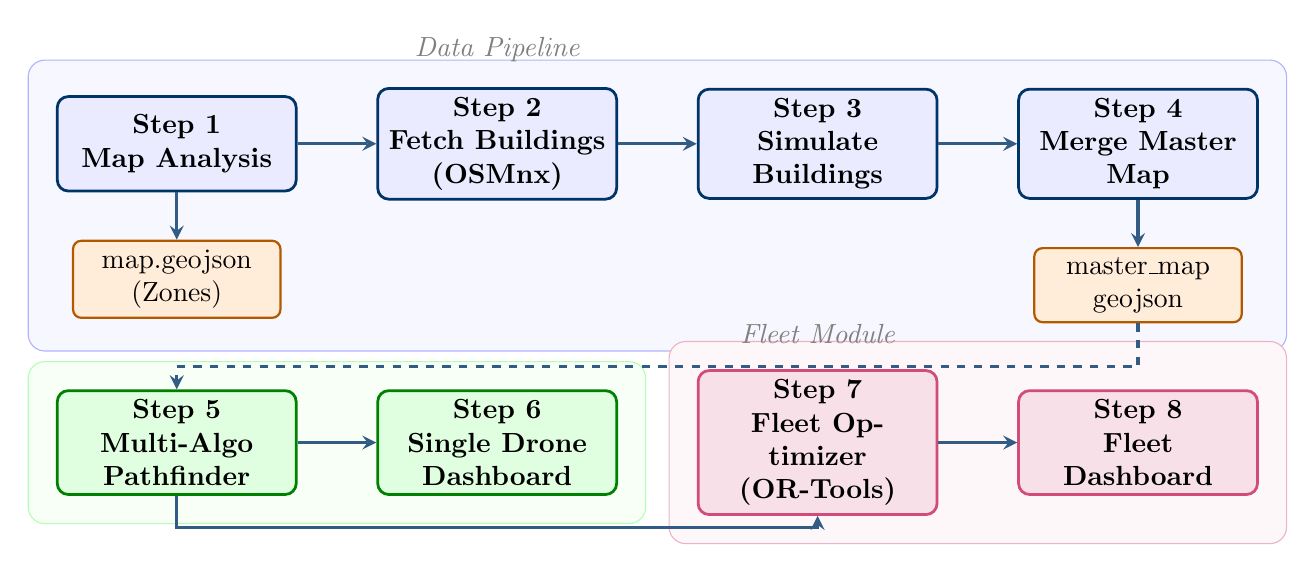
\begin{tikzpicture}[
    node distance=1.0cm and 1.0cm,
    block/.style={rectangle, draw=darkblue, line width=1pt, fill=blue!8, text width=2.8cm, text centered, rounded corners=4pt, minimum height=1.2cm, font=\normalsize\bfseries},
    greenblock/.style={rectangle, draw=green!50!black, line width=1pt, fill=green!12, text width=2.8cm, text centered, rounded corners=4pt, minimum height=1.2cm, font=\normalsize\bfseries},
    purpleblock/.style={rectangle, draw=purple!70, line width=1pt, fill=purple!12, text width=2.8cm, text centered, rounded corners=4pt, minimum height=1.2cm, font=\normalsize\bfseries},
    data/.style={rectangle, draw=orange!70!black, line width=0.8pt, fill=orange!15, text width=2.4cm, text centered, rounded corners=3pt, minimum height=0.9cm, font=\normalsize},
    arrow/.style={->, >=stealth, line width=1.2pt, draw=darkblue!80},
]

% Row 1: Data Pipeline
\node[block] (step1) {Step 1\\Map Analysis};
\node[block, right=of step1] (step2) {Step 2\\Fetch Buildings\\(OSMnx)};
\node[block, right=of step2] (step3) {Step 3\\Simulate\\Buildings};
\node[block, right=of step3] (step4) {Step 4\\Merge Master\\Map};

% Data nodes
\node[data, below=0.6cm of step1] (geojson) {map.geojson\\(Zones)};
\node[data, below=0.6cm of step4] (master) {master\_map\\geojson};

% Row 2: Engine + Dashboards
\node[greenblock, below=2.5cm of step1] (step5) {Step 5\\Multi-Algo\\Pathfinder};
\node[greenblock, right=of step5] (step6) {Step 6\\Single Drone\\Dashboard};
\node[purpleblock, right=of step6] (step7) {Step 7\\Fleet Optimizer\\(OR-Tools)};
\node[purpleblock, right=of step7] (step8) {Step 8\\Fleet\\Dashboard};

% Row 1 arrows
\draw[arrow] (step1) -- (step2);
\draw[arrow] (step2) -- (step3);
\draw[arrow] (step3) -- (step4);

% Data flow arrows
\draw[arrow] (step1) -- (geojson);
\draw[arrow] (step4) -- (master);
\draw[arrow, dashed] (master.south) -- ++(0,-0.55) -| (step5.north);

% Row 2 arrows
\draw[arrow] (step5) -- (step6);
\draw[arrow] (step5.south) -- ++(0,-0.4) -| (step7.south);
\draw[arrow] (step7) -- (step8);

% Labels
\node[above=0.2cm of step2, font=\normalsize\itshape, text=gray] {Data Pipeline};
\node[above=0.2cm of step7, font=\normalsize\itshape, text=gray] {Fleet Module};

% Grouping boxes
\scoped[on background layer]{
    \node[draw=blue!30, fill=blue!3, rounded corners=6pt, inner sep=10pt, fit=(step1)(step4)(geojson)(master)] {};
    \node[draw=green!30, fill=green!3, rounded corners=6pt, inner sep=10pt, fit=(step5)(step6)] {};
    \node[draw=purple!30, fill=purple!3, rounded corners=6pt, inner sep=10pt, fit=(step7)(step8)] {};
}

\end{tikzpicture}%
}
\caption{End-to-end system architecture showing the eight-stage processing pipeline from geospatial data ingestion to interactive fleet management dashboard.}
\label{fig:architecture}
\end{figure*}

\subsection{Data Acquisition and Processing (Steps 1--4)}

The pipeline begins with the ingestion of a custom GeoJSON file encoding the airspace classification for the Jaipur region. This file defines three zone categories:

\begin{itemize}[leftmargin=*]
    \item \textbf{Red Zones:} Strictly prohibited airspace surrounding airports, military installations, and government buildings. Height-encoded at 500\,m to guarantee pathfinder avoidance.
    \item \textbf{Yellow Zones:} Conditionally restricted areas near hospitals, schools, and religious sites. These require explicit operator permission; without it, they are treated identically to Red zones.
    \item \textbf{Boundary Zone:} A 20$\times$20\,km operational envelope centered on Jaipur ($26.757^\circ$--$26.937^\circ$N, $75.701^\circ$--$75.901^\circ$E).
\end{itemize}

Real building footprints are fetched via OSMnx from OpenStreetMap, augmented with a procedural generation module that creates approximately 1,000 additional buildings using Gaussian-clustered spatial distributions. Building heights follow a truncated normal distribution $\mathcal{N}(45, 10)$ within $[30, 60]$\,m. A minimum inter-building gap of 18\,m is enforced during placement.

All zone and building data are unified into a single master GeoJSON file where each feature carries a \texttt{height} attribute used by the pathfinding engine for altitude-aware obstacle classification.

\subsection{Grid Discretization and Obstacle Mapping (Step 5)}

The core navigation module discretizes the 20$\times$20\,km operational area into a grid with resolution $\Delta_{\text{lon}} = 0.0005^\circ$ ($\approx$50\,m) and $\Delta_{\text{lat}} = 0.00045^\circ$ ($\approx$50\,m), yielding a 401$\times$400 grid of 160,400 cells.

Each cell is classified as blocked or free based on:

{\small
\begin{equation}
\text{bl}(c) \!=\!
\begin{cases}
\text{T}, & c \in \mathcal{Z}_{r} \cup \mathcal{Z}_{y}^{\neg p} \\
\text{T}, & h(c) \geq h_d - m_s \\
\text{F}, & \text{otherwise}
\end{cases}
\label{eq:blocking}
\end{equation}
}

\noindent where $\text{bl}(c)$ denotes whether cell $c$ is blocked, $\mathcal{Z}_r$ and $\mathcal{Z}_y^{\neg p}$ represent Red and unpermitted Yellow zones, $h(c)$ is the obstacle height, $h_d$ is the drone cruise altitude, and $m_s$ is the vertical safety margin.

% ============================================================
% IV. METHODOLOGY
% ============================================================
\section{Methodology}

The pathfinding engine implements five distinct algorithms, each with different trade-offs between path optimality, computation speed, and exploration strategy. This section describes each algorithm and the common post-processing steps applied to all outputs.

\subsection{A* Search Algorithm}

A* \cite{hart1968astar} explores the grid by maintaining a priority queue ordered by the evaluation function:

\begin{equation}
f(n) = g(n) + h(n)
\end{equation}

\noindent where $g(n)$ is the accumulated cost from the start node and $h(n)$ is the heuristic estimate to the goal. The octile distance heuristic is employed for 8-directional movement:

\begin{equation}
h(n) = D_{\max} + (\sqrt{2} - 1) \cdot D_{\min}
\label{eq:octile}
\end{equation}

\noindent where $D_{\max} = \max(\Delta x, \Delta y)$ and $D_{\min} = \min(\Delta x, \Delta y)$. This heuristic is both admissible and consistent, guaranteeing optimal paths. A* balances exploration efficiency with path optimality, making it the recommended default algorithm for drone navigation.

\begin{algorithm}[!t]
\caption{A* Pathfinding with Obstacle Avoidance}
\label{alg:astar}
\begin{algorithmic}[1]
\STATE \textbf{Input:} Start $(s)$, Goal $(g)$, Grid $\mathcal{G}$
\STATE \textbf{Output:} Optimal path $\pi^*$ or $\varnothing$
\STATE Initialize open set $\mathcal{O} \leftarrow \{s\}$, $g(s) \leftarrow 0$
\WHILE{$\mathcal{O} \neq \varnothing$}
    \STATE $n \leftarrow \arg\min_{n \in \mathcal{O}} f(n)$
    \IF{$n = g$}
        \RETURN \textsc{ReconstructPath}$(n)$
    \ENDIF
    \FOR{each neighbor $n'$ of $n$}
        \IF{$\mathcal{G}[n'] = \text{blocked}$}
            \STATE \textbf{continue}
        \ENDIF
        \STATE $g' \leftarrow g(n) + \text{cost}(n, n')$
        \IF{$g' < g(n')$}
            \STATE Update $g(n'), f(n'), \text{parent}(n')$
            \STATE Add $n'$ to $\mathcal{O}$
        \ENDIF
    \ENDFOR
\ENDWHILE
\RETURN $\varnothing$
\end{algorithmic}
\end{algorithm}

\subsection{Best-First Search}

Best-First Search prioritizes nodes solely by their heuristic distance to the goal:

\begin{equation}
f(n) = h(n)
\end{equation}

\noindent Unlike A*, it ignores the accumulated path cost $g(n)$. This strategy aggressively expands nodes closer to the goal, resulting in the fastest computation among the tested algorithms. However, path optimality is not guaranteed---the algorithm may select longer routes by greedily pursuing the heuristic direction without considering detour costs already incurred.

\subsection{Breadth-First Search (BFS)}

BFS explores the grid in a level-order fashion using a FIFO queue. All nodes at distance $d$ from the start are expanded before any node at distance $d+1$. For uniform-cost grids, BFS guarantees the fewest-hop path. Its evaluation function is implicit:

\begin{equation}
f(n) = \text{depth}(n)
\end{equation}

\noindent BFS provides completeness---it will find a path if one exists---but does not use heuristic guidance. Consequently, it explores significantly more nodes than A* or Best-First Search, leading to higher computation times on large grids.

\subsection{Theta* (Any-Angle Pathfinding)}

Theta* \cite{nash2007theta} extends A* by permitting paths between any two nodes with unobstructed line-of-sight, not just grid-adjacent cells. During node expansion, Theta* checks whether a straight-line connection from the parent of the current node to the neighbor is obstacle-free using Bresenham's line algorithm:

\begin{equation}
f(n) = 
\begin{cases}
g(\text{parent}(s)) + c(\text{parent}(s), n) + h(n), & \text{if LOS} \\
g(s) + c(s, n) + h(n), & \text{otherwise}
\end{cases}
\end{equation}

\noindent where LOS denotes a clear line-of-sight between $\text{parent}(s)$ and $n$. This yields natively smoother, any-angle paths with fewer waypoints than grid-constrained algorithms, reducing the reliance on post-processing smoothing.

\subsection{RRT* (Optimal Rapidly-exploring Random Tree)}

RRT* \cite{karaman2011rrt} is a sampling-based planner that builds a tree by randomly sampling points in the configuration space and connecting them to the nearest existing node. It extends basic RRT with a rewiring step that optimizes connections within a radius $r$ of each new node:

\begin{equation}
r = \gamma \left(\frac{\log n}{n}\right)^{1/d}
\end{equation}

\noindent where $n$ is the number of nodes, $d$ is the space dimensionality, and $\gamma$ is a tuning constant. RRT* is asymptotically optimal---given sufficient iterations, it converges to the shortest path. However, it requires substantially more computation time compared to deterministic algorithms and its stochastic nature can lead to inconsistent results across runs.

\subsection{String-Pulling Path Smoothing}

All grid-based algorithms (A*, Best-First, BFS) produce jagged, grid-aligned paths. A string-pulling algorithm is applied as post-processing to reduce waypoints:

\begin{enumerate}[leftmargin=*]
    \item Start from the first waypoint.
    \item Test line-of-sight to the farthest subsequent waypoint.
    \item If the line is obstacle-free, skip all intermediate waypoints.
    \item Advance to the farthest visible waypoint and repeat.
\end{enumerate}

This reduces typical paths from 150+ waypoints to 4--8 smoothed waypoints, producing efficient straight-line flight segments suitable for drone autopilot systems.

\subsection{Single Drone Delivery}

In single drone mode, the operator specifies a pickup location (warehouse) and a delivery destination through the dashboard interface. The system performs the following steps:

\begin{enumerate}[leftmargin=*]
    \item \textbf{Coordinate Input:} The operator enters GPS coordinates manually or clicks on the interactive 2D map to set pickup and drop points.
    \item \textbf{Grid Conversion:} Input coordinates are converted to grid cell indices using the operational area bounds.
    \item \textbf{Obstacle Map Construction:} The master GeoJSON is loaded and all zone/building features are rasterized onto the grid. Yellow zones with operator permission are excluded from blocking.
    \item \textbf{Path Computation:} The selected algorithm (A*, Best-First, BFS, Theta*, or RRT*) computes a path on the obstacle grid.
    \item \textbf{Path Smoothing:} String-pulling reduces grid-aligned waypoints to smooth flight vectors.
    \item \textbf{Metric Calculation:} Path distance, travel time, detour ratio, and node count are computed and displayed.
\end{enumerate}

The computed path is visualized on a 2D Folium map showing zone boundaries and building footprints, and on a 3D PyDeck map with extruded building geometries. A compliance report confirms that no Red or unpermitted Yellow zones are intersected.

\subsection{Multi-Drone Fleet Delivery}

For scenarios requiring multiple simultaneous deliveries, the problem is formulated as a Capacitated Vehicle Routing Problem with Distance constraints (CVRPD). The fleet delivery workflow comprises three stages:

\subsubsection{Cost Matrix Construction}

A symmetric cost matrix $\mathbf{C} \in \mathbb{R}^{N \times N}$ is constructed where $C_{ij}$ is the A*-computed safe-path distance between locations $i$ and $j$:

\begin{equation}
C_{ij} = \text{A*\_dist}(l_i, l_j), \quad C_{ij} = C_{ji}
\end{equation}

For $N$ locations (1 warehouse + $N{-}1$ drops), this requires $\binom{N}{2}$ pathfinding computations. The obstacle map is built once and shared across all computations.

\subsubsection{OR-Tools VRP Formulation}

The optimization objective minimizes total fleet distance:

\begin{equation}
\min \sum_{k=1}^{M} \sum_{(i,j) \in \mathcal{R}_k} C_{ij}
\label{eq:vrp}
\end{equation}

\noindent subject to:
\begin{align}
& \sum_{j \in \mathcal{R}_k} d_j \leq Q_k, \quad \forall k \label{eq:capacity}\\
& \sum_{(i,j) \in \mathcal{R}_k} C_{ij} \leq R, \quad \forall k \label{eq:battery}\\
& \text{each drop visited exactly once} \label{eq:visit}\\
& \text{each route starts/ends at depot} \label{eq:depot}
\end{align}

\noindent where $M$ is the number of drones, $\mathcal{R}_k$ is the route of drone $k$, $d_j$ is the demand at drop $j$, $Q_k$ is the capacity, and $R = B_0 \times r$ is the maximum range (battery percentage $\times$ km per \%).

\subsubsection{Route Assignment and Visualization}

Google OR-Tools solves the VRP using PATH\_CHEAPEST\_ARC initialization followed by GUIDED\_LOCAL\_SEARCH improvement within a 10-second time limit. The solution assigns each delivery point to a specific drone, producing per-drone routes with distance, weight, and battery usage metrics. Each drone's flight path is visualized in a distinct color on the map.

% ============================================================
% V. IMPLEMENTATION
% ============================================================
\section{Implementation Details}

\subsection{Technology Stack}

Table~\ref{tab:techstack} summarizes the technologies employed across the system.

\begin{table}[!t]
\centering
\small
\caption{Technology Stack}
\label{tab:techstack}
\begin{tabular}{@{}p{2.6cm}p{4.2cm}@{}}
\toprule
\textbf{Component} & \textbf{Technology} \\
\midrule
Language & Python 3.11 \\
GIS Processing & GeoPandas, Shapely \\
Building Data & OSMnx (OpenStreetMap) \\
Pathfinding & Custom A*, BFS, Best-First, Theta*, RRT* \\
Fleet Optimization & Google OR-Tools 9.10 \\
Dashboard & Streamlit 1.55 \\
2D Visualization & Folium \\
3D Visualization & PyDeck \\
Spatial Math & NumPy, SciPy \\
\bottomrule
\end{tabular}
\end{table}

\subsection{Configurable Drone Parameters}

The system exposes operator-configurable parameters through the dashboard sidebar, listed in Table~\ref{tab:params}.

\begin{table}[!t]
\centering
\small
\caption{Operator-Configurable Drone Parameters}
\label{tab:params}
\begin{tabular}{@{}p{1.9cm}p{1.6cm}p{1.0cm}p{2.0cm}@{}}
\toprule
\textbf{Parameter} & \textbf{Range} & \textbf{Default} & \textbf{Effect} \\
\midrule
Altitude & 20--120\,m & 60\,m & Cruise height \\
Speed & 10--100\,km/h & 50\,km/h & Time est. \\
Vert.\ Margin & 0--30\,m & 10\,m & Above-bldg.\ gap \\
Bldg.\ Buffer & 0--20\,m & 3\,m & Lateral gap \\
Capacity & 0.5--20\,kg & 2.5\,kg & Max payload \\
Battery Rate & Fixed & 3\,km/\% & Discharge \\
\bottomrule
\end{tabular}
\end{table}

\subsection{Interactive Dashboard}

The system provides two operational modes through a unified Streamlit application, as shown in Fig.~\ref{fig:dashboard}:

\begin{enumerate}[leftmargin=*]
    \item \textbf{Single Drone Mode:} Operators specify pickup and drop coordinates, configure drone parameters and yellow zone permissions, select a pathfinding algorithm, and compute the optimal safe path with real-time 2D/3D visualization.
    
    \item \textbf{Multi-Drone Fleet Mode:} Operators define a warehouse and multiple drop points with delivery weights, configure fleet size and individual drone capacity, and invoke the OR-Tools optimizer. Results include per-drone route assignments with color-coded multi-path visualization.
\end{enumerate}

\begin{figure}[!t]
\centering
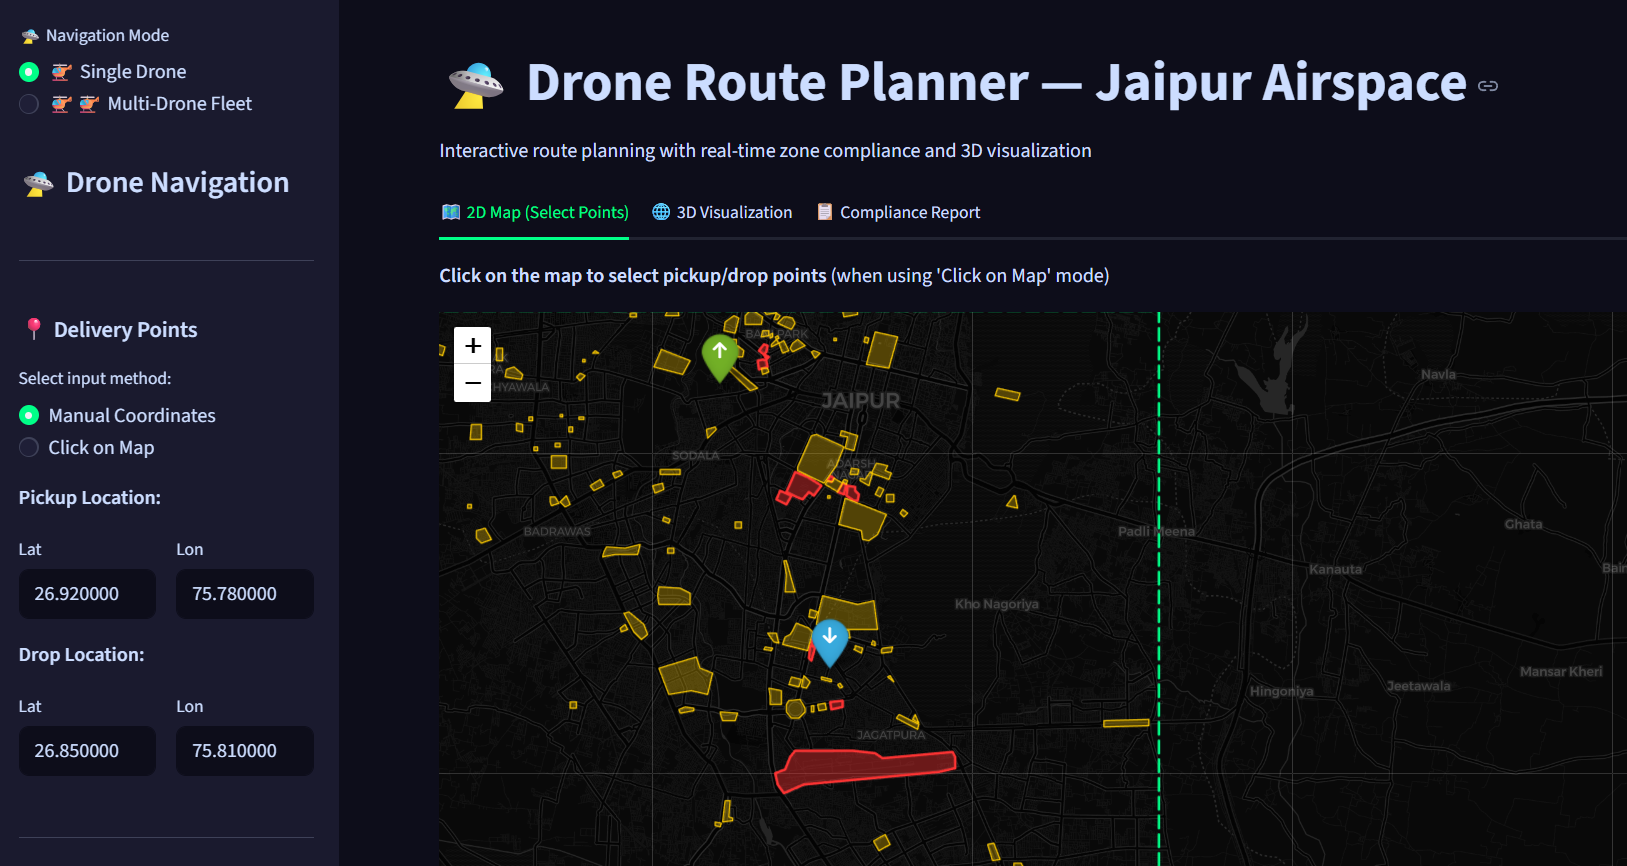
\includegraphics[width=\columnwidth]{Dashboard.png}
\caption{Single Drone Mode dashboard showing the interactive route planning interface with 2D map, coordinate input panel, and algorithm selection in the sidebar.}
\label{fig:dashboard}
\end{figure}

\begin{figure}[!t]
\centering
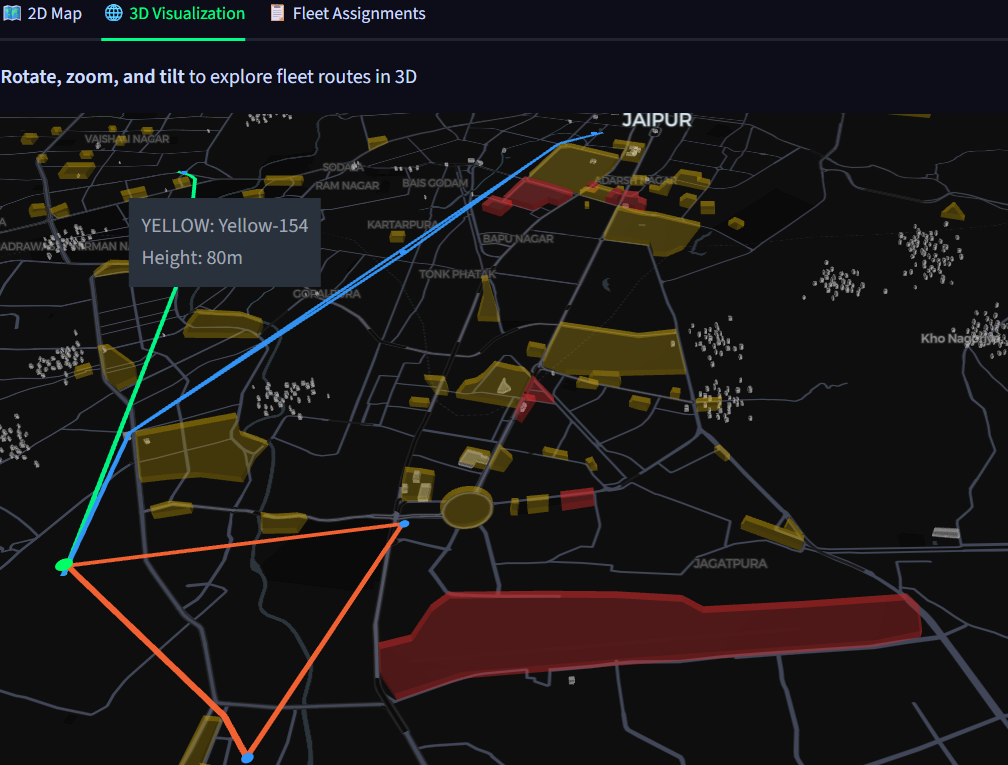
\includegraphics[width=\columnwidth]{3D_Map.png}
\caption{3D visualization of multi-drone fleet routes over the Jaipur airspace. Building obstacles (gold), Red zones (red), and drone flight paths (colored lines) are rendered with extruded geometries on a dark basemap.}
\label{fig:3dmap}
\end{figure}

% ============================================================
% VI. EXPERIMENTAL RESULTS
% ============================================================
\section{Experimental Results}

\subsection{Test Environment}

Experiments were conducted over the Jaipur operational area with the configuration detailed in Table~\ref{tab:env}.

\begin{table}[!t]
\centering
\small
\caption{Experimental Environment Configuration}
\label{tab:env}
\begin{tabular}{@{}p{3.2cm}p{3.8cm}@{}}
\toprule
\textbf{Parameter} & \textbf{Value} \\
\midrule
Operational Area & 20 $\times$ 20\,km \\
Grid Resolution & 50\,m $\times$ 50\,m \\
Grid Dimensions & 401 $\times$ 400 (160,400 cells) \\
Red Zones & 12 (airports, govt.\ bldgs.) \\
Yellow Zones & 109 (hospitals, schools) \\
Simulated Buildings & 1,079 \\
Building Heights & 30--60\,m (truncated normal) \\
Drone Altitude & 60\,m (default) \\
Safety Margin & 10\,m (default) \\
\bottomrule
\end{tabular}
\end{table}


\subsection{Algorithm Comparison}

All five pathfinding algorithms were benchmarked across five diverse scenarios spanning the Jaipur operational area: North-to-South long traverse, East-to-West medium traverse, short hop between nearby points, diagonal long-distance route, and city-center traverse. Table~\ref{tab:comparison} presents the aggregated results.

\begin{table}[H]
\centering
\caption{Pathfinding Algorithm Comparison (5 Scenarios)}
\label{tab:comparison}
\resizebox{\columnwidth}{!}{%
\begin{tabular}{@{}lcccc@{}}
\toprule
\textbf{Algorithm} & \textbf{Success} & \textbf{Avg Dist} & \textbf{Avg Time} & \textbf{Nodes} \\
 & \textbf{Rate} & \textbf{(m)} & \textbf{(s)} & \textbf{Explored} \\
\midrule
\textbf{A*} & \textbf{5/5} & \textbf{8,438} & \textbf{0.051} & \textbf{151} \\
Best-First & 5/5 & 8,510 & 0.019 & 154 \\
BFS & 5/5 & 8,473 & 0.296 & 151 \\
Theta* & 5/5 & 8,459 & 0.173 & 1,066 \\
RRT* & 3/5 & 10,736 & 48.84 & 13,997 \\
\bottomrule
\end{tabular}%
}
\end{table}

\subsubsection{Key Findings}

\textbf{A*} achieves the shortest average path distance (8,438\,m) with a computation time of 51\,ms and explores only 151 nodes per run, establishing it as the best overall algorithm for grid-based drone navigation. Its combination of heuristic guidance and accumulated cost tracking yields optimal paths efficiently.

\textbf{Best-First Search} is the fastest algorithm (19\,ms average) but produces slightly longer paths (8,510\,m) due to the absence of cost accumulation. It is suitable when computation speed is prioritized over path optimality.

\textbf{BFS} finds paths of comparable quality to A* (8,473\,m) but requires 5.8$\times$ more computation time (296\,ms) due to exhaustive level-order exploration without heuristic guidance.

\textbf{Theta*} produces smooth any-angle paths (8,459\,m) with native smoothness, reducing dependence on post-processing. However, line-of-sight checks increase node exploration to 1,066 per run.

\textbf{RRT*} achieves a 60\% success rate with significantly higher computation time (48.84\,s) and path distance (10,736\,m). Its stochastic sampling makes it unreliable for real-time grid-based applications but valuable in high-dimensional continuous spaces.

\subsection{Comparison Visualizations}

Figures~\ref{fig:comp_distance}--\ref{fig:comp_success} present the algorithm comparison results graphically across four key metrics.

\begin{figure}[H]
\centering
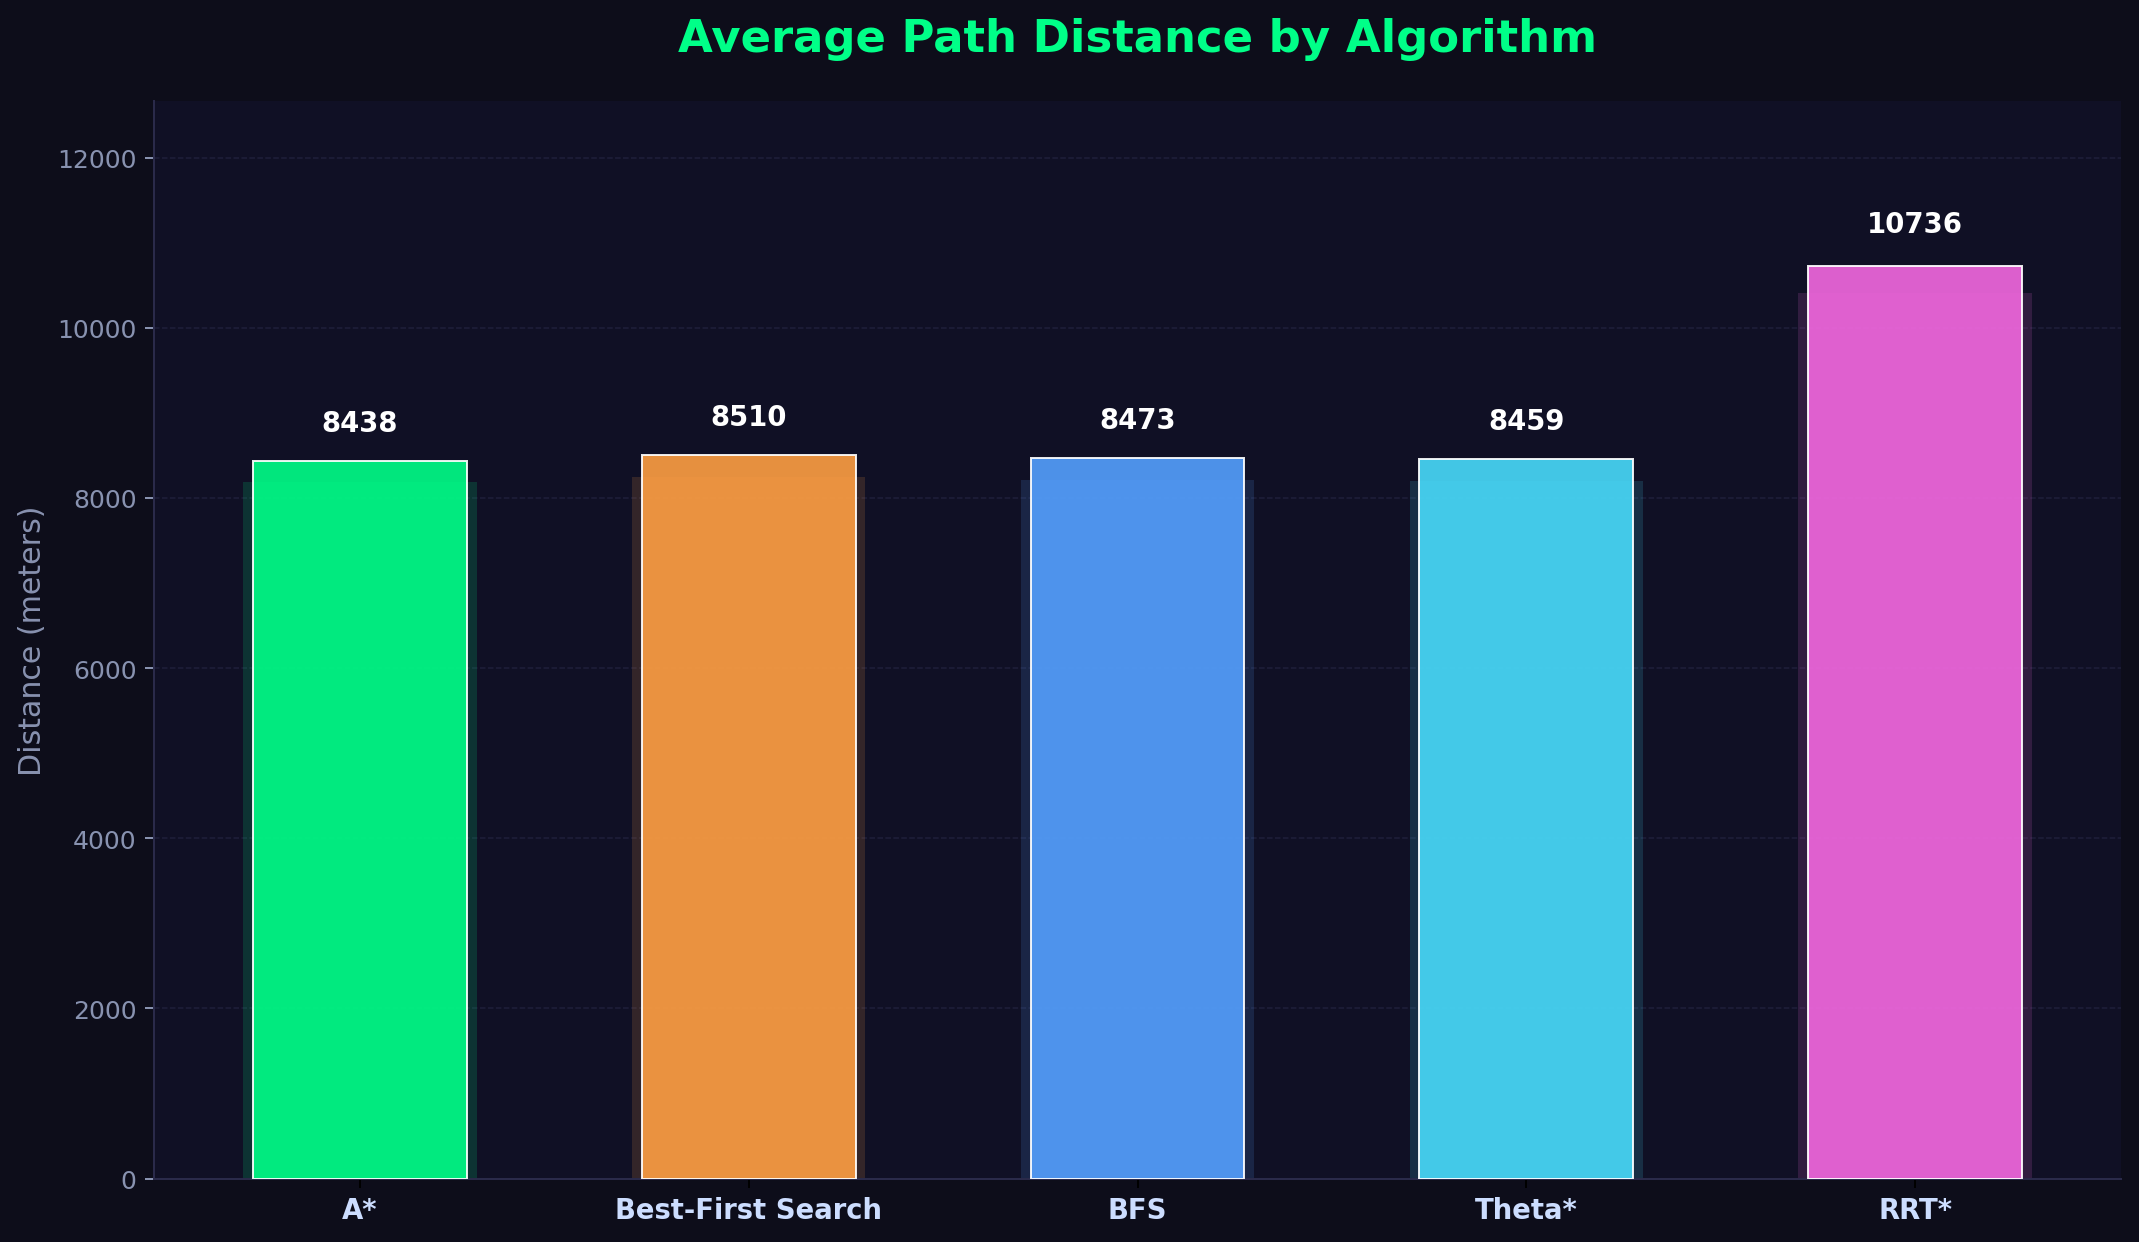
\includegraphics[width=\columnwidth]{comparison_path_distance.png}
\caption{Average path distance comparison. A* produces the shortest paths (8,438\,m), while RRT* generates 27\% longer routes.}
\label{fig:comp_distance}
\end{figure}

\begin{figure}[H]
\centering
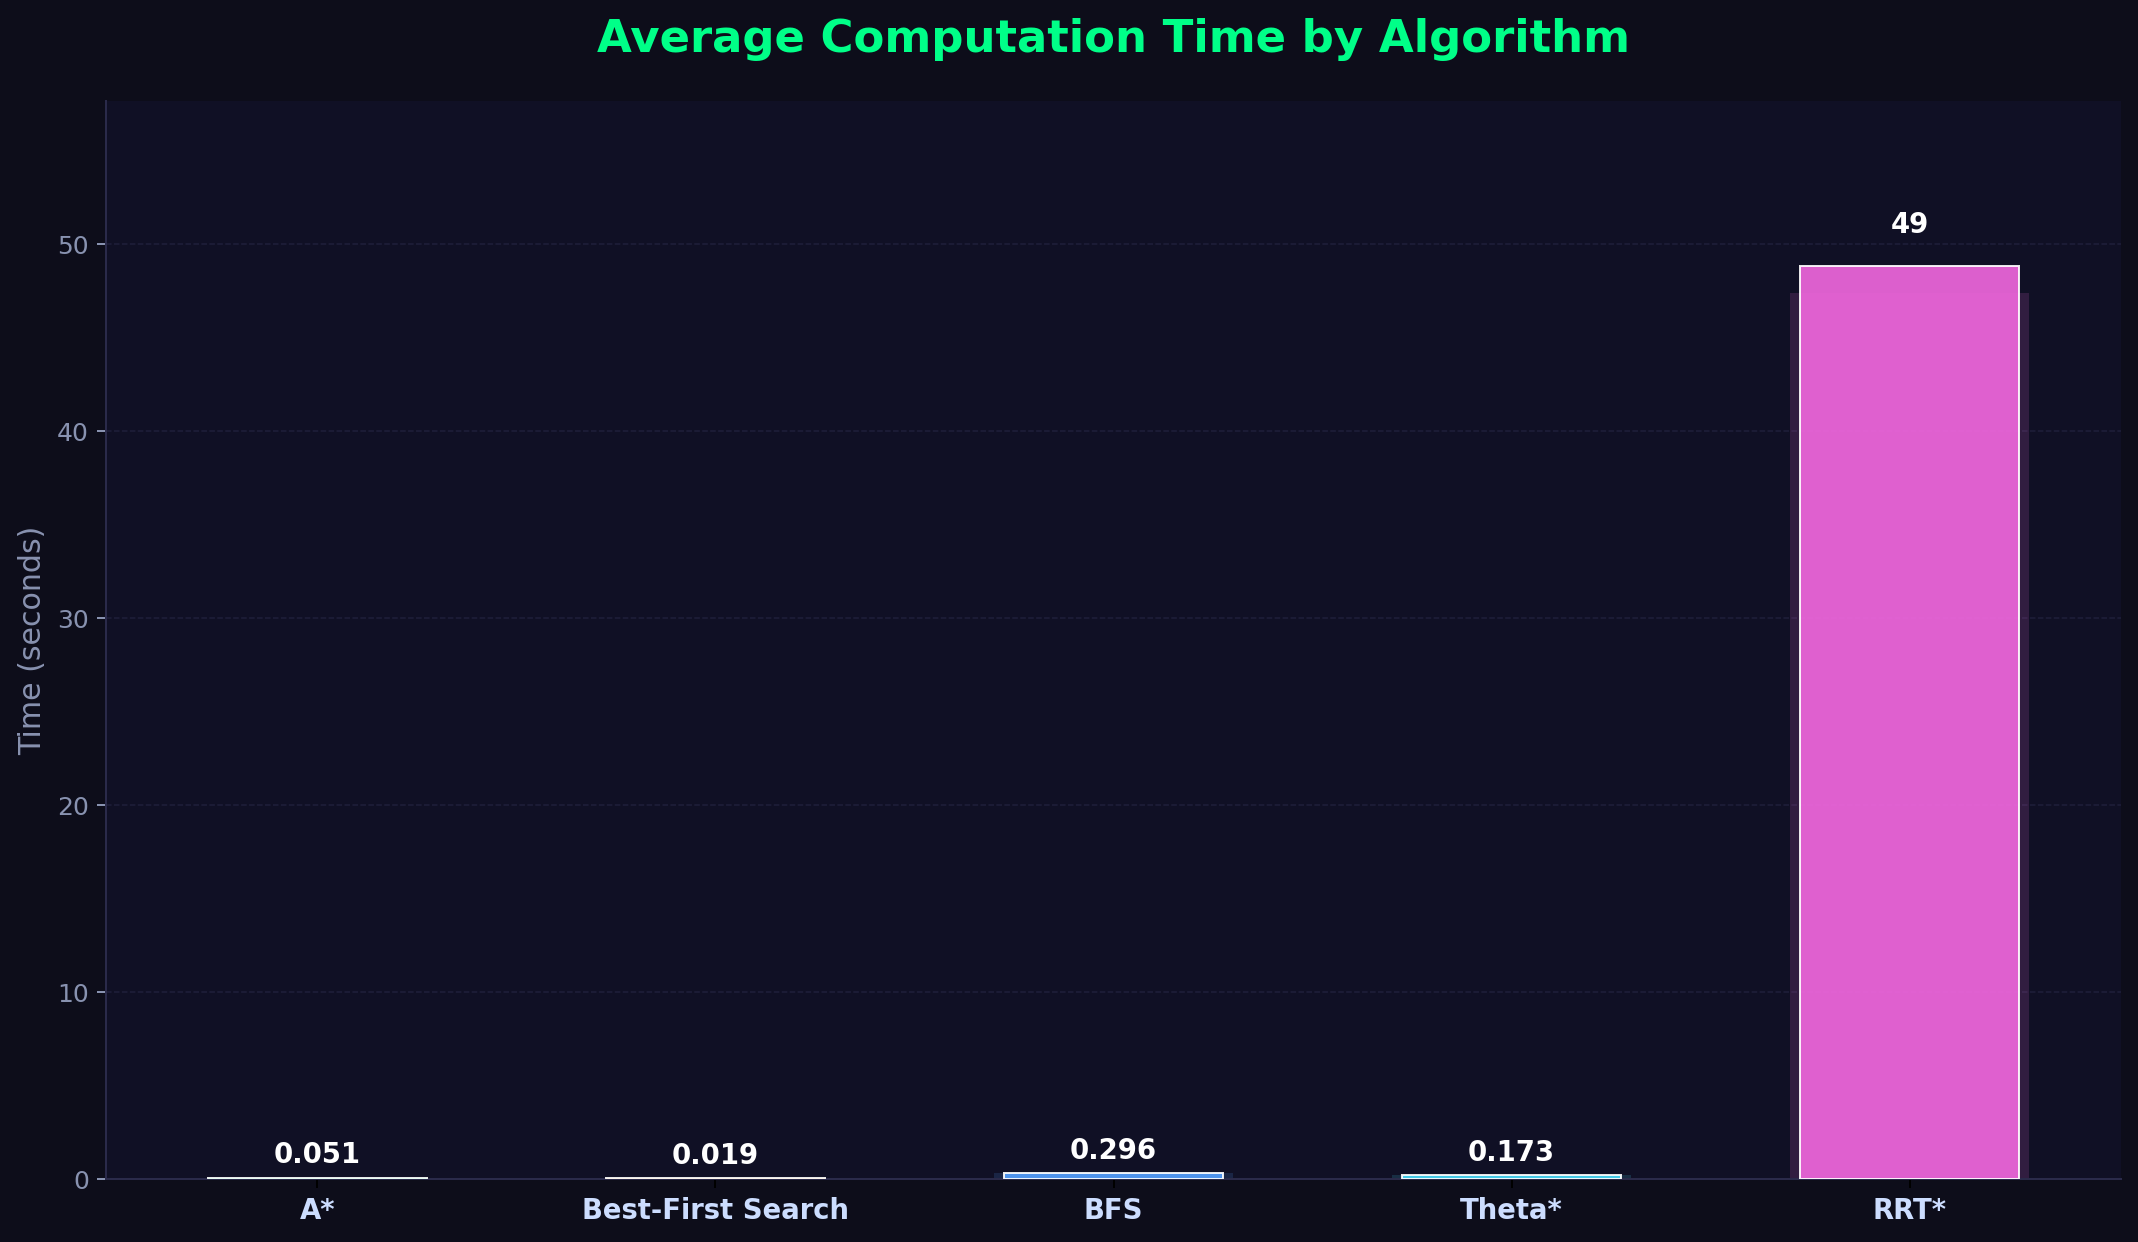
\includegraphics[width=\columnwidth]{comparison_computation_time.png}
\caption{Average computation time. Best-First Search is fastest (0.019\,s), while RRT* requires 48.84\,s.}
\label{fig:comp_time}
\end{figure}

\begin{figure}[H]
\centering
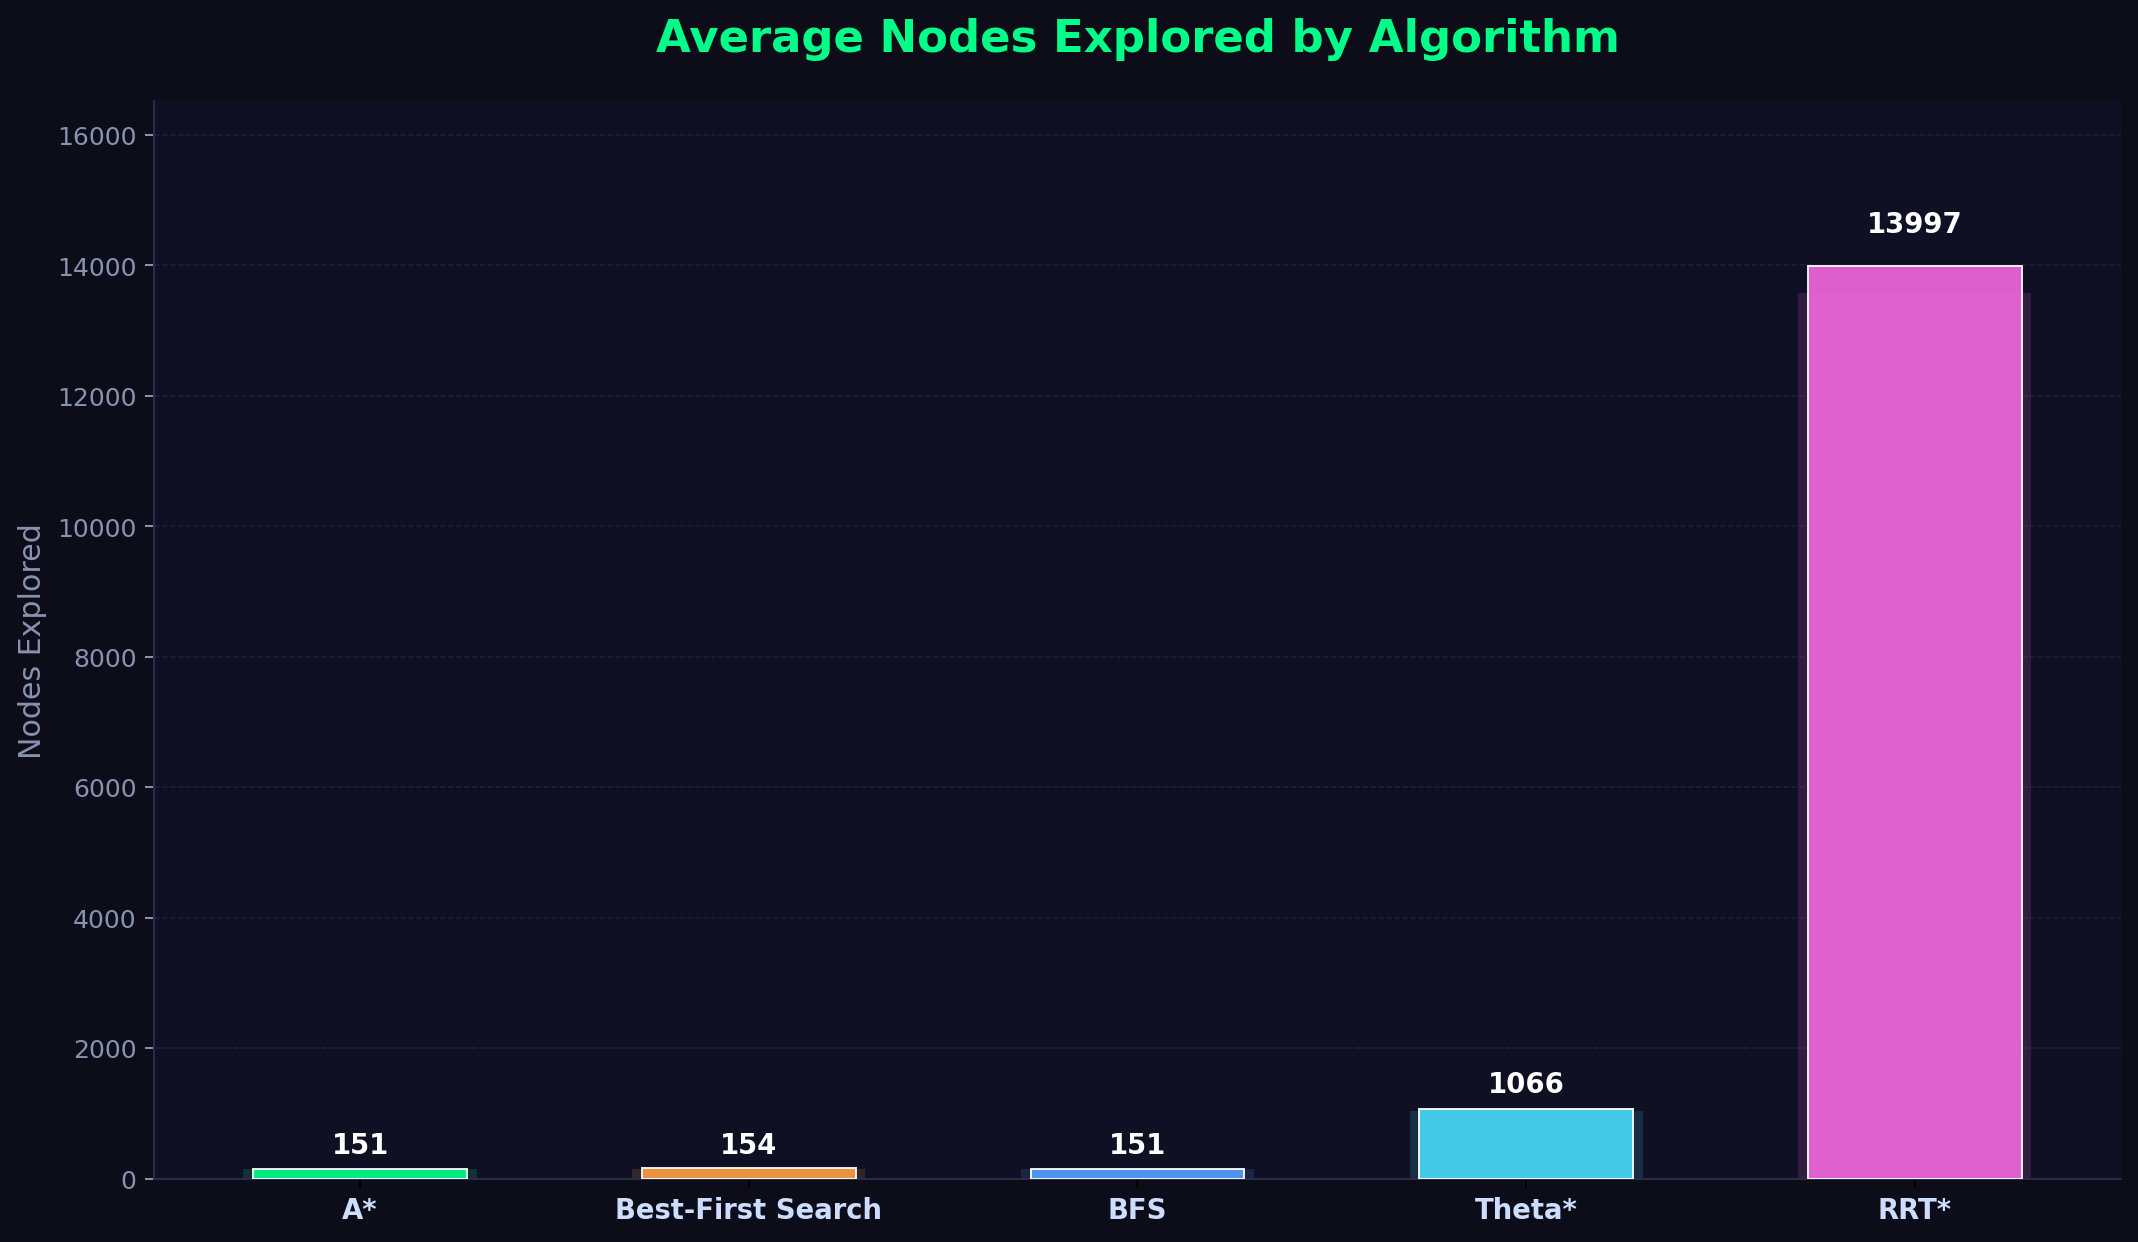
\includegraphics[width=\columnwidth]{comparison_nodes_explored.png}
\caption{Nodes explored per algorithm. A* and BFS explore $\sim$151 nodes, Theta* 1,066, and RRT* 13,997.}
\label{fig:comp_nodes}
\end{figure}

\begin{figure}[H]
\centering
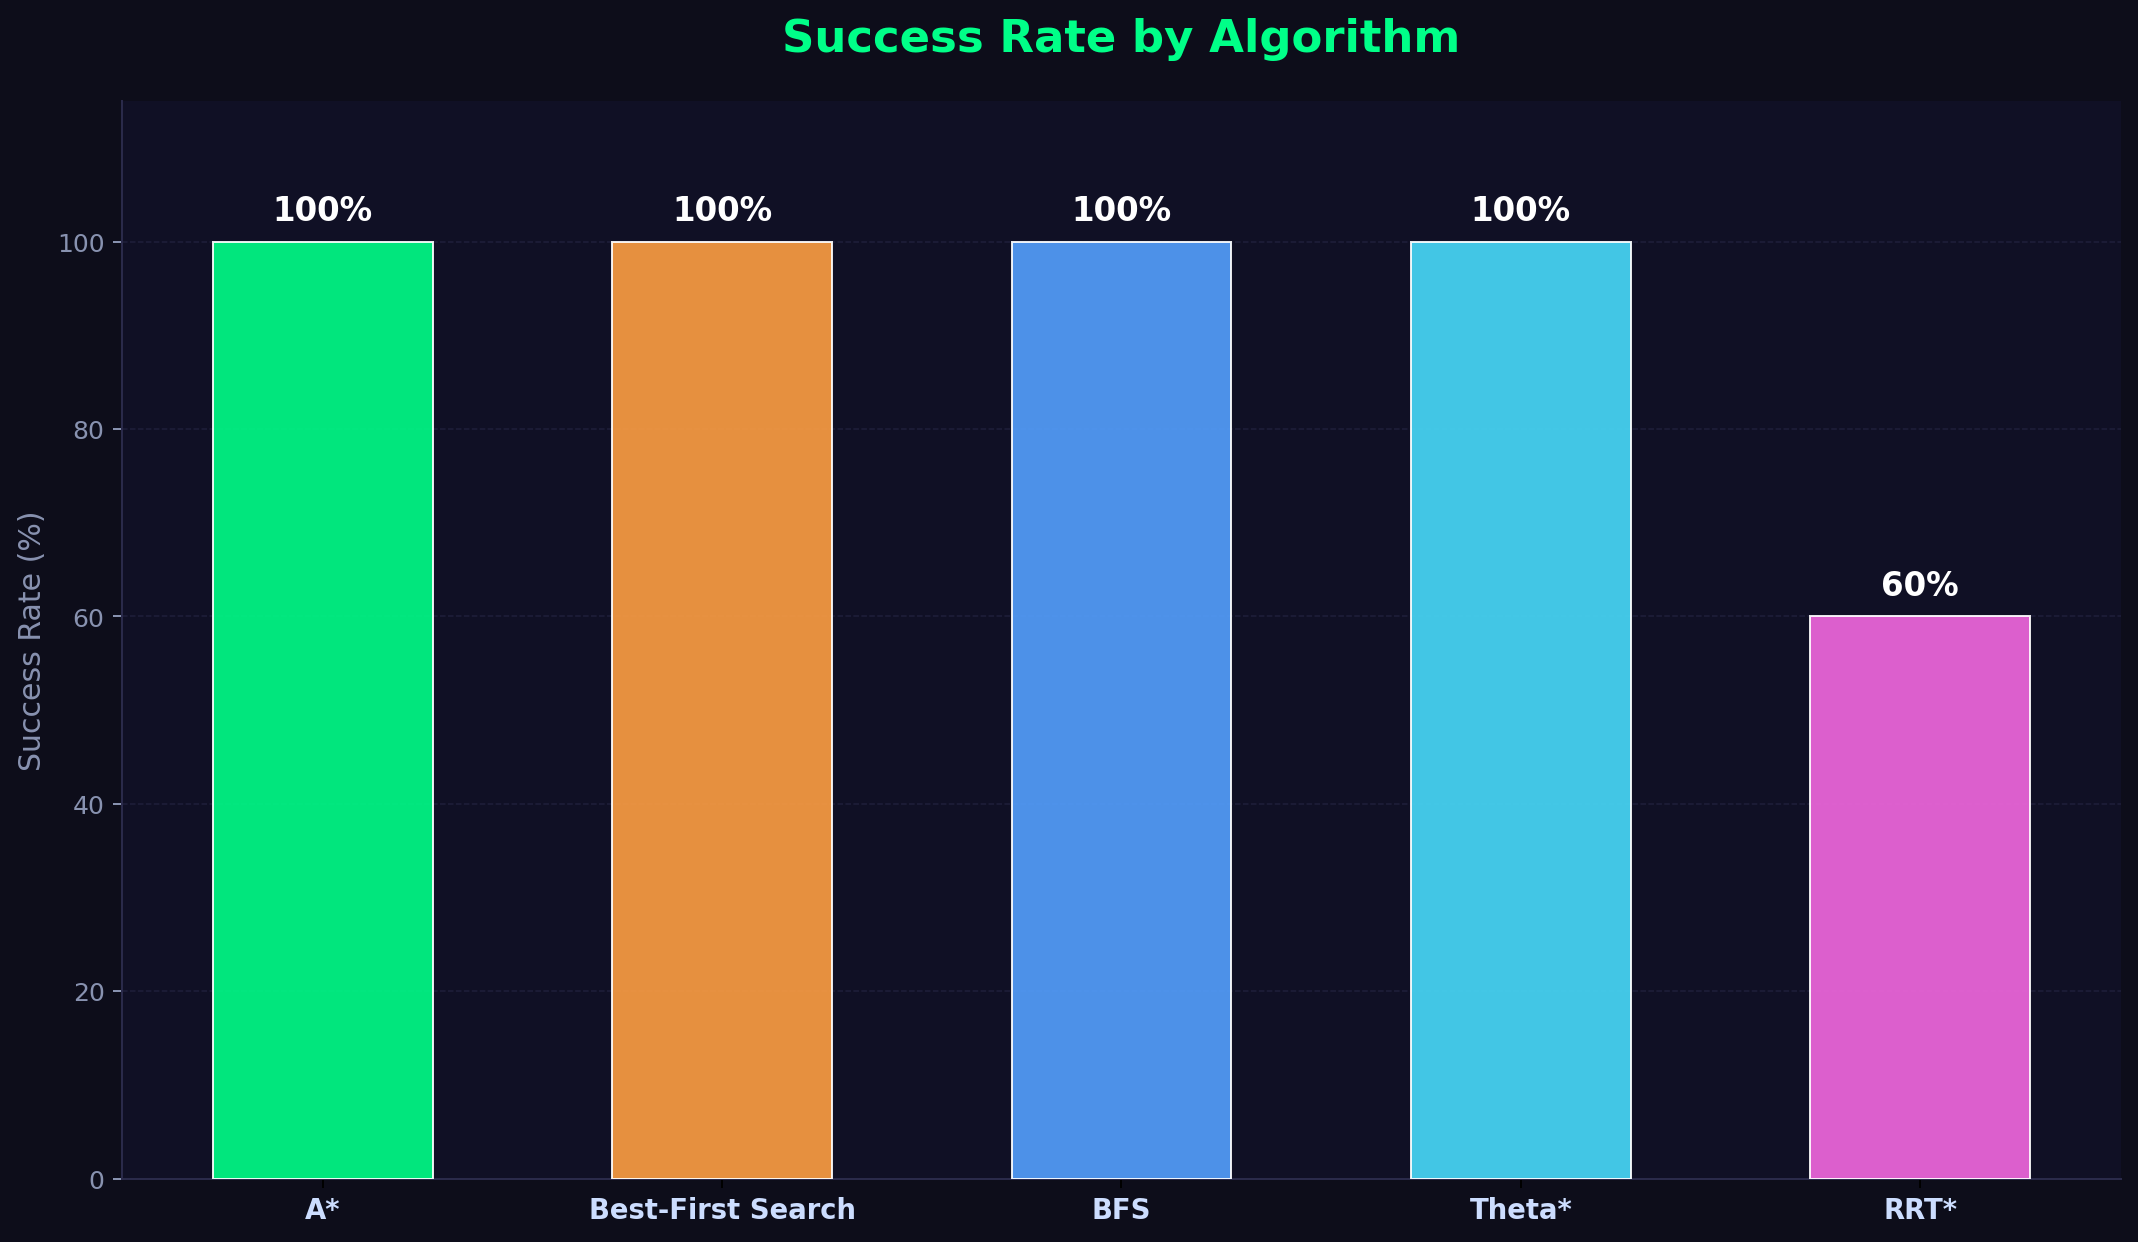
\includegraphics[width=\columnwidth]{comparison_success_rate.png}
\caption{Algorithm success rate. All deterministic algorithms achieve 100\%, RRT* fails in 2 of 5 scenarios.}
\label{fig:comp_success}
\end{figure}

\subsection{Path Smoothing Effectiveness}

The string-pulling step consistently reduces waypoint counts by 95--97\%, as shown in Table~\ref{tab:smoothing}.

\begin{table}[!t]
\centering
\small
\caption{Path Smoothing Effectiveness (A* Algorithm)}
\label{tab:smoothing}
\begin{tabular}{@{}lccc@{}}
\toprule
\textbf{Scenario} & \textbf{Raw WPs} & \textbf{Smoothed} & \textbf{Reduction} \\
\midrule
N$\to$S Long & 156 & 6 & 96.2\% \\
E$\to$W Medium & 201 & 4 & 98.0\% \\
Short Hop & 30 & 4 & 86.7\% \\
Diagonal Long & 246 & 5 & 98.0\% \\
City Center & 121 & 3 & 97.5\% \\
\bottomrule
\end{tabular}
\end{table}

\subsection{Fleet Optimization Results}

A fleet optimization scenario with 1 warehouse, 5 delivery points, and 3 drones was evaluated. Table~\ref{tab:fleet} presents per-drone assignment results.

\begin{table}[!t]
\centering
\small
\caption{Fleet Optimization Results (5 Drops, 3 Drones)}
\label{tab:fleet}
\begin{tabular}{@{}lcccc@{}}
\toprule
\textbf{Drone} & \textbf{Drops} & \textbf{Dist.} & \textbf{Wt.} & \textbf{Batt.} \\
 & & (km) & (kg) & Used \\
\midrule
Drone 1 & D2, D5 & 22.31 & 2.3 & 7.4\% \\
Drone 2 & D1, D3 & 28.14 & 2.1 & 9.4\% \\
Drone 3 & D4 & 16.71 & 0.5 & 5.6\% \\
\midrule
\textbf{Total} & \textbf{5/5} & \textbf{67.16} & \textbf{4.9} & -- \\
\bottomrule
\end{tabular}
\end{table}

All five deliveries were assigned across three drones, with the maximum single-drone battery usage at 9.4\%, well within the 300\,km theoretical range. The OR-Tools solver converged within 10 seconds. Fig.~\ref{fig:3dmap} shows the resulting multi-drone flight paths visualized in 3D.

% ============================================================
% VII. DISCUSSION
% ============================================================
\section{Discussion}

\subsection{Algorithm Selection Guidance}

Based on the experimental results, the following selection guidance is proposed:

\begin{itemize}[leftmargin=*]
    \item \textbf{A* (Recommended Default):} Best overall balance of path optimality and computation speed. Suitable for all standard delivery scenarios.
    \item \textbf{Best-First Search:} Preferred when sub-20\,ms response is required and minor path suboptimality is acceptable.
    \item \textbf{BFS:} Useful as a baseline for path quality validation; impractical for real-time use on large grids.
    \item \textbf{Theta*:} Preferred when smooth, any-angle paths are desired without post-processing, particularly for autopilot systems that follow waypoints precisely.
    \item \textbf{RRT*:} Suitable only for offline planning in continuous 3D spaces where deterministic grid methods are infeasible.
\end{itemize}

\subsection{Regulatory Compliance Validation}

The system was validated against all 12 Red and 109 Yellow zones in the Jaipur airspace. In all tested scenarios, no computed path intersected a Red zone. Yellow zone traversal occurred only when explicit operator permission was granted, verified through post-hoc geometric intersection testing.

\subsection{Limitations}

\begin{enumerate}[leftmargin=*]
    \item \textbf{Static Environment:} Dynamic obstacles (other drones, birds) are not modelled.
    \item \textbf{Constant Altitude:} The drone flies at a fixed cruise altitude without altitude variation along the route.
    \item \textbf{Wind Effects:} Meteorological conditions affecting flight time and battery consumption are not incorporated.
    \item \textbf{Grid Resolution:} The 50\,m grid may miss narrow gaps in densely packed areas.
\end{enumerate}

% ============================================================
% VIII. DEPLOYMENT
% ============================================================
\section{Deployment}

The complete system is deployed as a public Streamlit application on Hugging Face Spaces, accessible at:

\begin{center}
\small\url{https://huggingface.co/spaces/harphool17/drone-route-planner}
\end{center}

The deployment packages all source code, pre-computed geospatial data, and dependencies into a containerized environment. Users interact through a browser-based interface without requiring local installation of Python, GIS software, or any additional libraries. The sidebar mode selector enables seamless switching between single-drone navigation and multi-drone fleet planning modes.

% ============================================================
% IX. CONCLUSION AND FUTURE WORK
% ============================================================
\section{Conclusion and Future Work}

This paper presented a regulation-compliant drone delivery route planning system for Indian urban environments. The multi-algorithm pathfinding engine was evaluated across five algorithms, with A* emerging as the recommended choice due to its optimal balance of path quality (8,438\,m average), computation speed (51\,ms), and 100\% reliability. The fleet optimization module successfully assigned delivery tasks under payload and battery constraints using Google OR-Tools, converging within 10 seconds.

Future directions include:

\begin{enumerate}[leftmargin=*]
    \item \textbf{Dynamic Obstacle Integration:} Real-time ADS-B data for moving obstacle avoidance.
    \item \textbf{3D Path Planning:} Altitude-varying paths using layered grids or RRT* in 3D space.
    \item \textbf{Weather-Aware Routing:} Weather API integration for wind-adjusted battery models.
    \item \textbf{Multi-Depot VRP:} Support for multiple warehouse locations.
    \item \textbf{Machine Learning Enhancement:} Neural heuristic functions trained on historical delivery data.
\end{enumerate}

% ============================================================
% REFERENCES
% ============================================================
\bibliographystyle{IEEEtranN}

\begin{thebibliography}{25}

\bibitem{amazon2022prime}
Amazon Prime Air, ``Drone delivery service,'' Amazon, 2022. [Online]. Available: \url{https://www.amazon.com/Amazon-Prime-Air/}

\bibitem{dgca2021}
Directorate General of Civil Aviation, ``The Drone Rules, 2021,'' Ministry of Civil Aviation, Government of India, 2021.

\bibitem{khatib1986potential}
O. Khatib, ``Real-time obstacle avoidance for manipulators and mobile robots,'' \textit{Int.\ J.\ Robotics Research}, vol.~5, no.~1, pp.~90--98, 1986.

\bibitem{bortoff2000path}
S. A. Bortoff, ``Path planning for UAVs,'' in \textit{Proc.\ American Control Conf.}, Chicago, IL, 2000, pp.~364--368.

\bibitem{ergezer2013}
H. Ergezer and K. Leblebicioglu, ``3D path planning for UAVs for maximum information collection,'' in \textit{Unmanned Aircraft Systems (ICUAS)}, Atlanta, GA, 2013, pp.~370--377.

\bibitem{karaman2011rrt}
S. Karaman and E. Frazzoli, ``Sampling-based algorithms for optimal motion planning,'' \textit{Int.\ J.\ Robotics Research}, vol.~30, no.~7, pp.~846--894, 2011.

\bibitem{nash2007theta}
A. Nash, K. Daniel, S. Koenig, and A. Felner, ``Theta*: Any-angle path planning on grids,'' in \textit{Proc.\ AAAI Conf.\ Artificial Intelligence}, 2007, pp.~1177--1183.

\bibitem{dantzig1959truck}
G. B. Dantzig and J. H. Ramser, ``The truck dispatching problem,'' \textit{Management Science}, vol.~6, no.~1, pp.~80--91, 1959.

\bibitem{ortools2023}
Google, ``OR-Tools: Google optimization tools,'' 2023. [Online]. Available: \url{https://developers.google.com/optimization}

\bibitem{murray2015flying}
C. C. Murray and A. G. Chu, ``The flying sidekick traveling salesman problem: Optimization of drone-assisted parcel delivery,'' \textit{Transportation Research Part C}, vol.~54, pp.~86--109, 2015.

\bibitem{priyadarshini2022drone}
R. Priyadarshini, P. Kumar, and S. Mishra, ``Drone path planning with no-fly zone avoidance for Indian urban airspace,'' in \textit{IEEE Int.\ Conf.\ Computing, Communication and Security}, 2022, pp.~1--6.

\bibitem{hart1968astar}
P. E. Hart, N. J. Nilsson, and B. Raphael, ``A formal basis for the heuristic determination of minimum cost paths,'' \textit{IEEE Trans.\ Systems Science and Cybernetics}, vol.~4, no.~2, pp.~100--107, 1968.

\bibitem{dijkstra1959}
E. W. Dijkstra, ``A note on two problems in connexion with graphs,'' \textit{Numerische Mathematik}, vol.~1, no.~1, pp.~269--271, 1959.

\bibitem{aggarwal2020path}
S. Aggarwal and N. Kumar, ``Path planning techniques for unmanned aerial vehicles: A review, solutions, and challenges,'' \textit{Computer Communications}, vol.~149, pp.~270--299, 2020.


\bibitem{shakhatreh2019unmanned}
H. Shakhatreh \textit{et al.}, ``Unmanned aerial vehicles (UAVs): A survey on civil applications and key research challenges,'' \textit{IEEE Access}, vol.~7, pp.~48572--48634, 2019.

\bibitem{macrina2020drone}
G. Macrina, L. Di Puglia Pugliese, F. Guerriero, and G. Laporte, ``Drone-aided routing: A literature review,'' \textit{Transportation Research Part C: Emerging Technologies}, vol.~120, p.~102762, 2020.

\bibitem{mohsan2022towards}
S. A. H. Mohsan, N. Q. H. Othman, Y. Li, M. H. Alsharif, and M. A. Khan, ``Unmanned aerial vehicles (UAVs): Practical aspects, applications, open challenges, security issues, and future trends,'' \textit{Intelligent Service Robotics}, vol.~16, pp.~109--137, 2023.

\bibitem{toth2014vehicle}
P. Toth and D. Vigo, \textit{Vehicle Routing: Problems, Methods, and Applications}, 2nd ed. Philadelphia, PA: SIAM, 2014.

\bibitem{harabor2011jps}
D. Harabor and A. Grastien, ``Online graph pruning for pathfinding on grid maps,'' in \textit{Proc.\ AAAI Conf.\ Artificial Intelligence}, 2011, pp.~1114--1119.

\bibitem{geojson2016}
H. Butler, M. Daly, A. Doyle, S. Gillies, S. Hagen, and T. Schaub, ``The GeoJSON format,'' IETF, RFC~7946, Aug.\ 2016. [Online]. Available: \url{https://tools.ietf.org/html/rfc7946}

\end{thebibliography}
\end{document}
